\section{Ciclo de refrigeración por compresión}

\subsection{Elementos fundamentales}

Los sistemas de refrigeranción por compresión constan, básicamente, de cuatro elementos que consideramos fundamentales a través de los cuales circula un fluido refrigerante.

Estos elementos son:

\begin{enumerate}
	\item Compresor
	\item Condensador
	\item Dispositivo de expansión
	\item Evaporador
\end{enumerate}

\begin{figure}[h]
	\centering
	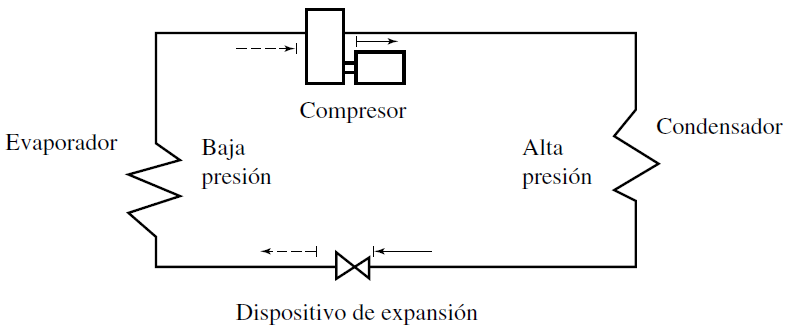
\includegraphics[width=\textwidth]{figuras/elementos fundamentales.png}
	\caption{Elementos fundamentales de un sistema de refrigeración}
	\label{fig:elementos_fundamentales}
\end{figure}


\subsubsection{Funciones principales}

La función de cada uno de ellos es la siguiente:

\textbf{Compresor:}

Aspira el fluido refrigerante a la presión de baja establecida y lo comprime elevando su presión y temperatura hasta unos valores tales que se pueda efectuar la condensación. La descarga la efectua en el condensador.

\textbf{Condensador:}

Es el elemento de la instalación que se encarga de pasar el estado de vapor del fluido refrigerante a estado líquido. El fluido refrigerante entra en el condensador en estado de gas (vapor recalentado) y sale en estado líquido a la temperatura que se condensó o incluso a una temperatura menor si se produce subenfriamiento.

\textbf{Dispositivo de expansión:}

Hace que el fluido, que entra en estado líquido, sufra una caída de presión (y temperatura) hasta la necesaria en el evaporador. También controla la cantidad de fluido refrigerante que debe entrar en el evaporador.

\textbf{Evaporador:}

Se encarga de enfriar o acondicionar la cámara. Puede estar dentro o fuera de la misma. Su misión es que el fluido refrigerante, que entra a baja presión y temperatura, efectúe el enfriamiento.\\
Es el elemento de la instalación donde el fluido refrigerante se evapora, tomando calor del exterior del evaporador debido a la diferencia de temperaturas.

\subsubsection{Fluido refrigerante}

El fluido refrigerante está sometido a cambios de estado a lo largo del circuito:

\begin{itemize}
	\item En el compresor entra en estado de gas, a baja presión y temperatura, y sale con presión y temperatura más altas (recalentado), que es como entra en el condensador.
	\item Del condensador sale estado líquido y entra dispositivo de expansión.
	\item Del dispositivo de expansión sale en forma de mezcla de líquido y gas (expansión), a baja presión y temperatura, y entra en el evaporador.
	\item Del evaporador sale en estado de gas, a baja presión y temperatura, de donde es aspirado por el compresor, y se inicia el nuevo ciclo.
\end{itemize}

Como sabemos, \textit{al aumentar la presión de un fluido se eleva su punto de ebullición, y al disminuir la presión, también disminuye su punto de ebullición.} Esta es una de las claves de la refrigeración.

\subsection{Alta y baja presión}

Debemos diferenciar la parte del circuito que está sometida a una presión alta y la que se encuentra a baja presión (\autoref{fig:elementos_fundamentales}).

\textit{La parte correspondiente a la alta presión está comprendida entre la descarga del compresor y la entrada del dispositivo de expansión.}

Hay que resaltar que la temperatura del fluido refrigerante no es la misma en todo ese tramo:

\begin{itemize}
	\item Entre la salida del compresor y la entrada del condensor el fluido está en estado de gas (gas recalentado).
	\item Se condensa a una temperatura menor y s desde el vale del condensador a esa misma temperatura o menor si se subenfría, con lo cual, la temperaturadel fluido a la entrada del dispositivo de expansión puede ser igual o menor que la de condensación.
\end{itemize}

\textit{La parte que corresponde a la baja presión, es la comprendida entre la salida del dispositivo de expansión y la entrada del compresor.}

La instalación dispone del manoómetro de baja presión para conocer su valor en cada momento. En este tramo, también la temperatura varía (aumenta) desde el evaporador hasta la entrada del compresor.

\subsection{Elementos de seguridad y control}

La \autoref{fig:elementos_seguridad_y_control} representa los cuatro elementos fundamentales para el estudio de sus principales características a los que se añaden los elementos de seguridad y control.

\begin{figure}[H]
	\centering
	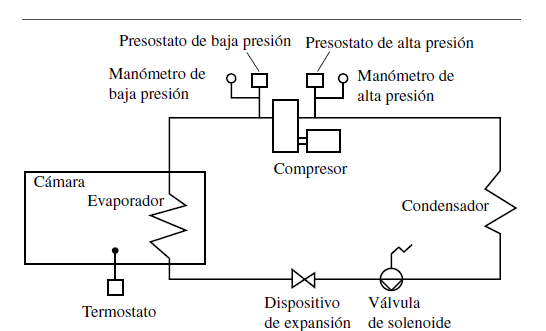
\includegraphics[width=\textwidth]{Elementos_seguridad_y_control.png}
	\caption{Elementos fundamentales de un circuito frigorífico en los que se añaden los dispositivos de seguridad y control.}
	\label{fig:elementos_seguridad_y_control}
\end{figure}

\subsubsection{Presostatos}

Son unos aparatos que, activados por presión, tienen la función de abrir o cerrar un circuito mediante uno o varios contactos normalmente ya sean abiertos o cerrados. De manera práctica, se puede decir que son unos interruptores eléctricos que funcionan por presión. Pueden ser:

\begin{enumerate}
	[a.]
	\item Presostatos de alta presión 
	
	Se conecten a la descarga del compresor, y su función es impedir que en la zona de alta presión, se alcancen valores que afecten al rendimiento de la instalación o a la propia seguridad de las personas. Se regulan a una determinada presión, y cuando la instalación alcanza ese valor, entonces el presostato para el compresor.
	\item Presostatos de baja presión
	
	Se conectan a la aspiración del compresor, y función es evitar que la presión, en la zona baja, pueda ``caer'' por debajo de la presión atmosférica y evitar también que la presión descienda por debajo de la normal de funcionamiento, ya que afectaría al rendimiento. De hecho, su regulación debe estar \textit{siempre} por encima de la presión atmosférica. Cuando la presión descienda hasta la correspondiente al valor de regulación, el presostato parará el compresor. 
\end{enumerate}

Los presostatos de alta y baja presión no tienen que instalarse necesariamente por separado, ya que también se puede instalar los dos formando un solo elemento, llamado \textit{presostato combinado}, tal como se representa en la \autoref{fig:Presostato combinado}.

\begin{figure}[H]
	\centering
	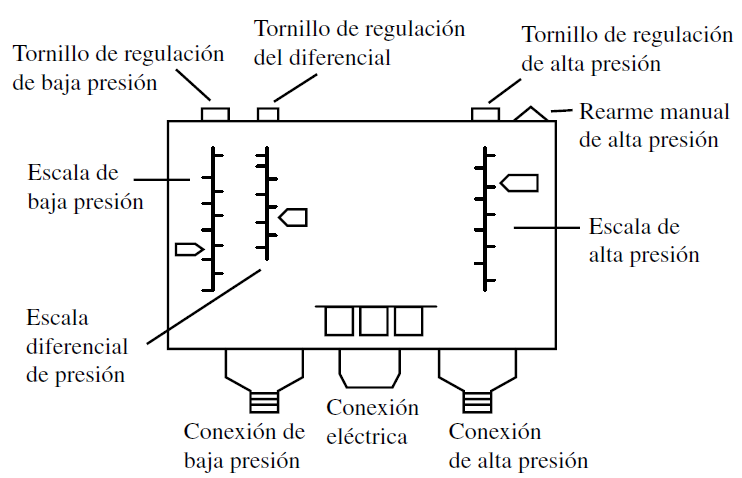
\includegraphics[width=\textwidth]{figuras/presostato combinado.png}
	\caption{Presostato combinado}
	\label{fig:Presostato combinado}
\end{figure}

\subsubsection{Termostato}

Es el elemento que controla la temperatura de la cámara. Abre o cierra un contacto conectado a un circuito eléctrico cuando alcanza la temperatura de regulación. Se puede decir que es un interruptor o conmutador eléctrico que funciona por temperatura.

El termostato con depósito de gas, se basa en que éste sufre variaciones de presión en relación a la temperatura que rodea al depósito que lo contiene. Si una de las paredes del depósitoes de membrana, sufrirá deformaciones a consecuencia de esos cambios de temperatura. Si además actúa sobre unos contactos, bien sea directa o inderectamente, los abrirá o cerrará de acuerdo a la regulación establecida. 

Como los presostatos, disponen de un diferencial (diferencia entre las temperaturas de arranque y de paro) que puede ser fijo o variable. Por lo general suele ser de $\pm 3$.

\textbf{Ejemplo de aplicación}

Queremos mantener una temperatura de -20 \textcelsius en la cámara y el diferencial establecido es de $\pm 3$ \textcelsius.

Ello quiere decir que la instalción se parará cuando la temperatura alcance los -23 \textcelsius, pues el termostato, en ese momento, cerrará la válvula de solenoide. Debido a la transmisión de calor, la temperatura en el interior de la cámara aumentará hasta alcanzar los -17 \textcelsius y entonces el termostato abrirá la válvula de la solenoide, y se pondrá de nuevo en funcionamiento el compresor.

\subsubsection{Válvula de solenoide (o electroválvula)}

Aunque no es un elemento de regulación ni de control, debemos comentar sus principales características para poder enterder mejor el siguiente apartado.

Su funcionamiento es de todo o nada, no es de regulación proporcional. Cuando está activada por el campo magnético, levanta el vástago de la válvula y deja pasar el fluido. Cuando se desactiva, cesa la imanación (no hay campo magnético), el vástago de la válvula cae y corta el paso del fluido refrigerante.

Va conectada en serie con el termostato, por decirlo de una mnera práctica; el termostato deja pasar o corta la corriente eléctrica a la bobina, con lo cual la válvula se abre o cierra, según las necesidades térmicas.


\begin{figure}[H]
	\centering
	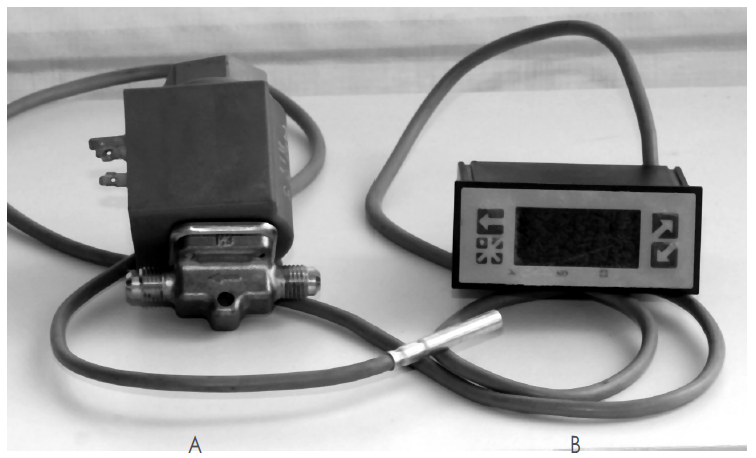
\includegraphics[width=\textwidth]{figuras/solenoide y termometro.png}
	\caption{A: Válvula de solenoide. B:Termostato electrónico}
	\label{fig:solenoide y termostato}
\end{figure}

\subsubsection{Presostato diferencial de aceite}

Es un elemento de seguridad; de hecho es un interruptor de seguridad (\autoref{fig:Presostato diferencial de aceite}). PRotege al compresor contra una presión de aceite demasiado baja. Se conecta a la aspiración y a la descarga de la bomba de lubricación.

\begin{figure}[H]
	\centering
	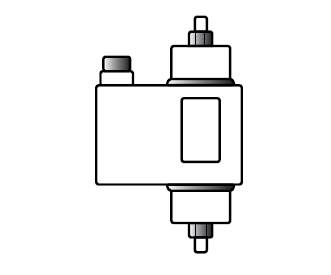
\includegraphics[width=6cm, height=6cm]{figuras/Presostato diferencial de aceite.png}
	\caption{Presostato diferencial de aceite}
	\label{fig:Presostato diferencial de aceite}
\end{figure}

\subsection{Elementos complementarios}
Una instalación podría trabajar con los elementos anteriormente citados, pero, evidentemente, necesita de otros elementos complementarios para que el ciclo de trabajo se pueda efectuar con el mayor rendimiento posible. 

En el siguiente esquema (\autoref{fig:Instalacion con elementos complementarios} se representan los más importantes y su disposición en las instalaciones.)

\begin{figure}[H]
	\centering
	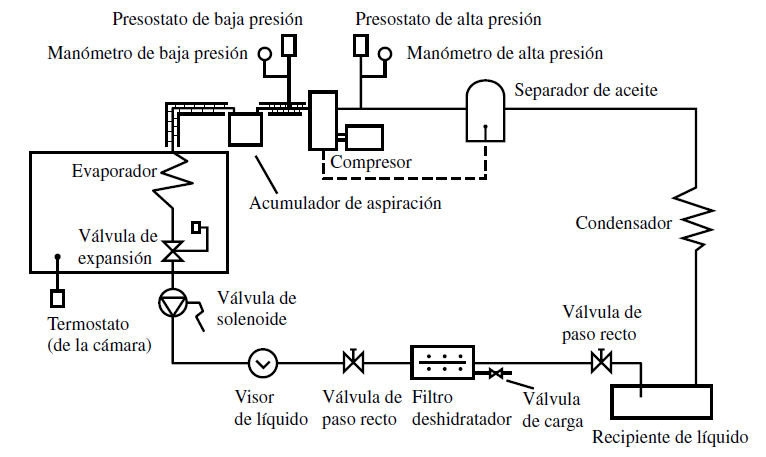
\includegraphics[width=\textwidth]{figuras/Instalación con elementos complementarios.png}
	\caption{Instalación de los elementos fundamentales, de seguridad y control, y complementarios}
	\label{fig:Instalacion con elementos complementarios}
\end{figure}

\subsubsection{Resistencia calefactora (del cárter)}

Cuando las temperaturas que rodean al compresor (temperatura ambiente) son muy bajas, en los tiempos de parada del compresor puede ocurrir que el fluido refrigerante depositado en el cárter se condense, por lo que en el momento del arranque se produce una vaporización rápida del fluido que conlleva un arrastre de aceite.

También la baja temperatura ambiente afecta a la viscosidad del aceite, ya que si es muy baja, ésta aumenta las resistencias a vencer en el arranque. Para evitar estas circunstancias se instalan en el cárter unas peque\~{n}a resistencias eléctricas que lo mantienen a cierta temperatura, de tal manera que cuando para el compresor, entran en funcionamiento.

\subsubsection{Separador de aceite}

Se instala en la tubería de descarga, después del compresor. El fluido refrigerante sale del compresor mezclado con el aceite de lubricación y éste debe retornar al cárter principalmente por dos razones:

\begin{enumerate}
	[1.]
	\item  porque el nivel de aceite del cárter iría disminuyendo y
	\item porque el aceite, cuando llegue al circuito de baja presión, podría tener problemas de retorno (deja de ser miscible y crea problemas en los evaporadores, por ejemplo de transmisión o taponamientos)
\end{enumerate}

Los hay de varios tipos. Por ejemplo los que aprovechan la fuerza centrífuga de la descarga del compresor para efectuar la separación (Figura \ref{fig:Separador de aceite}) o bien la caída de velocidad a la entrada del separador para efectuar la separación.

%     LO DEJO COMENTADO PORQUE DESP TE LO QUIERO MOSTRAR A VER SI VOS SABES QUE PASA
%	Si recortamos las imágenes como para que quede centrado el objeto, mejor :)
\begin{wrapfigure}{r}{0.4\linewidth}
	\centering
	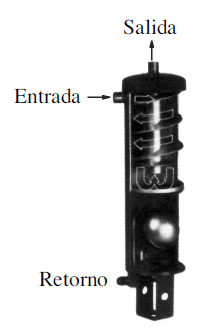
\includegraphics[width=.5\linewidth]{figuras/separador de aceite.png}
	\caption{Separador de aceite}
	\label{fig:Separador de aceite}
\end{wrapfigure}  

El aceite se va decantando en el fondo del separador hasta alcanzar un nivel tal que el regulador, por ejemplo un flotador de nivel, lo detecta y abre el paso de retorno hacia el cárter.

Una representación del retorno de aceite se puede observar en la \autoref{fig:Línea de retorno de aceite}.


Cuando el nivel de aceite en el interior del separador alcanza el nivel estipulado, el regulador de nivel abre la electroválvula y el aceite retorna al cárter. El aceite retorna porque la presión en el interior del separador (presión de alta) es superior a la presión reinante en el cárter.

No tienen una eficacia del 100\%, pero es bueno que una pequeña cantidad de aceite circule por la instalación ya que mantiene engrasados elementos como válvulas, electroválvulas, etc.

\begin{figure}[h]
	\centering
	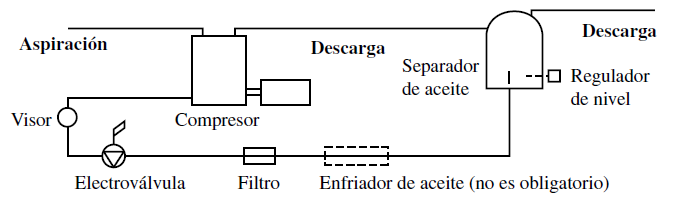
\includegraphics[width=.9\linewidth]{figuras/Linea de retorno de aceite.png}
	\caption{Línea de retorno de aceite}
	\label{fig:Línea de retorno de aceite}
\end{figure}

\subsubsection{Recipiente de líquido}

Se coloca a la salida del condensador, aunque los hay del tipo condensador-recipiente que forman un solo elemento.

El líquido que sale del condensador no va directamente al evaporador, salvo si se utilizan tubos capolares, sino que se ``almacena'' en el recipiente. Mantiene una reserva de líquido para restituirlo según la demanda. Los hay horizontales (\autoref{fig:Recipiente de líquido horizontal}) y (\autoref{fig:Recipiente de líquido vertical}) verticales.

Su capacidad varía con las características de la instalación; si se trata de una con varios evaporadores, su capacidad será por lo menos 1,25 veces la capacidad del evaporador mayor.

\begin{figure}[H]
	\centering
	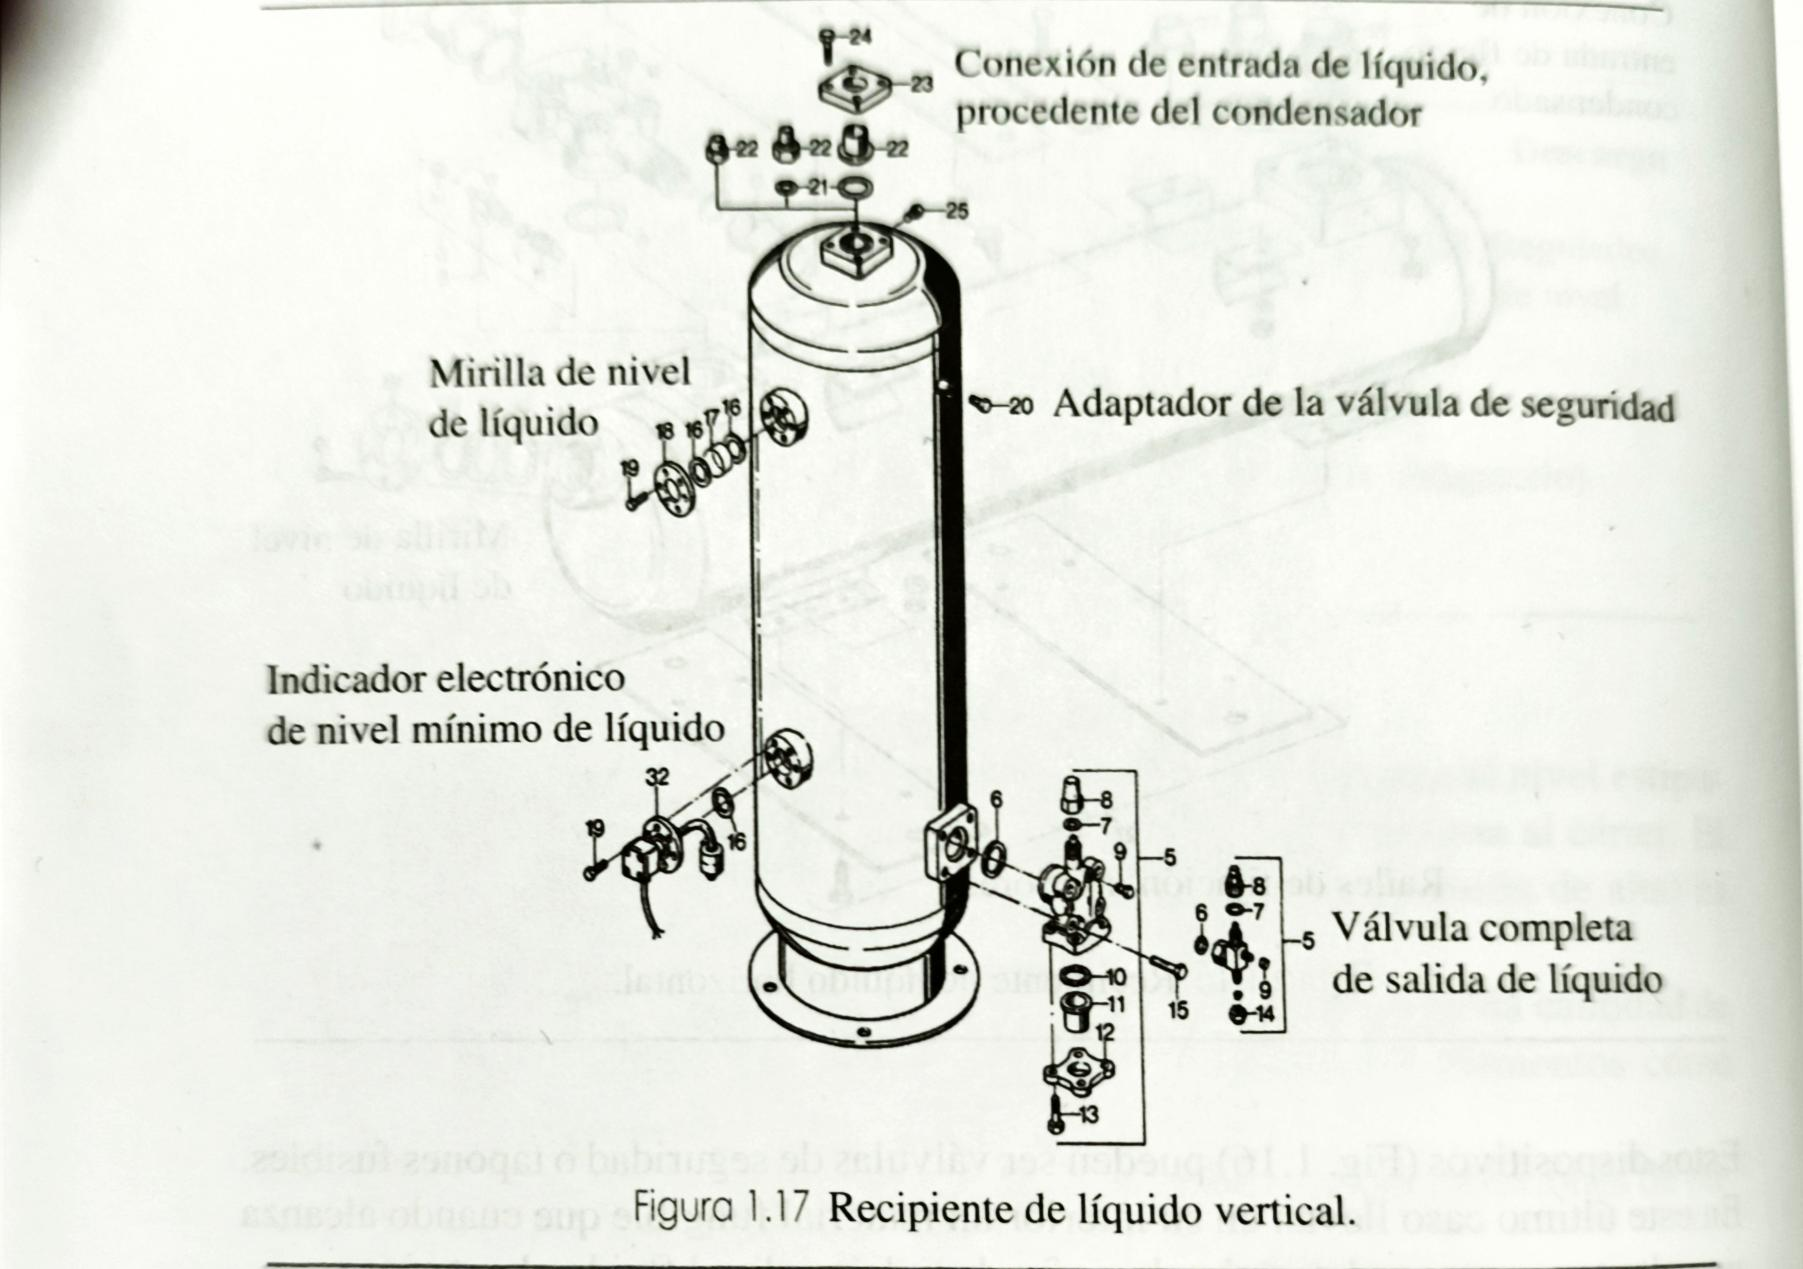
\includegraphics[width=0.7\textwidth]{figuras/recipiente vertical.jpg}
	\caption{Recipiente de líquido vertical}
	\label{fig:Recipiente de líquido vertical}
\end{figure}

\begin{figure}[H]
	\centering
	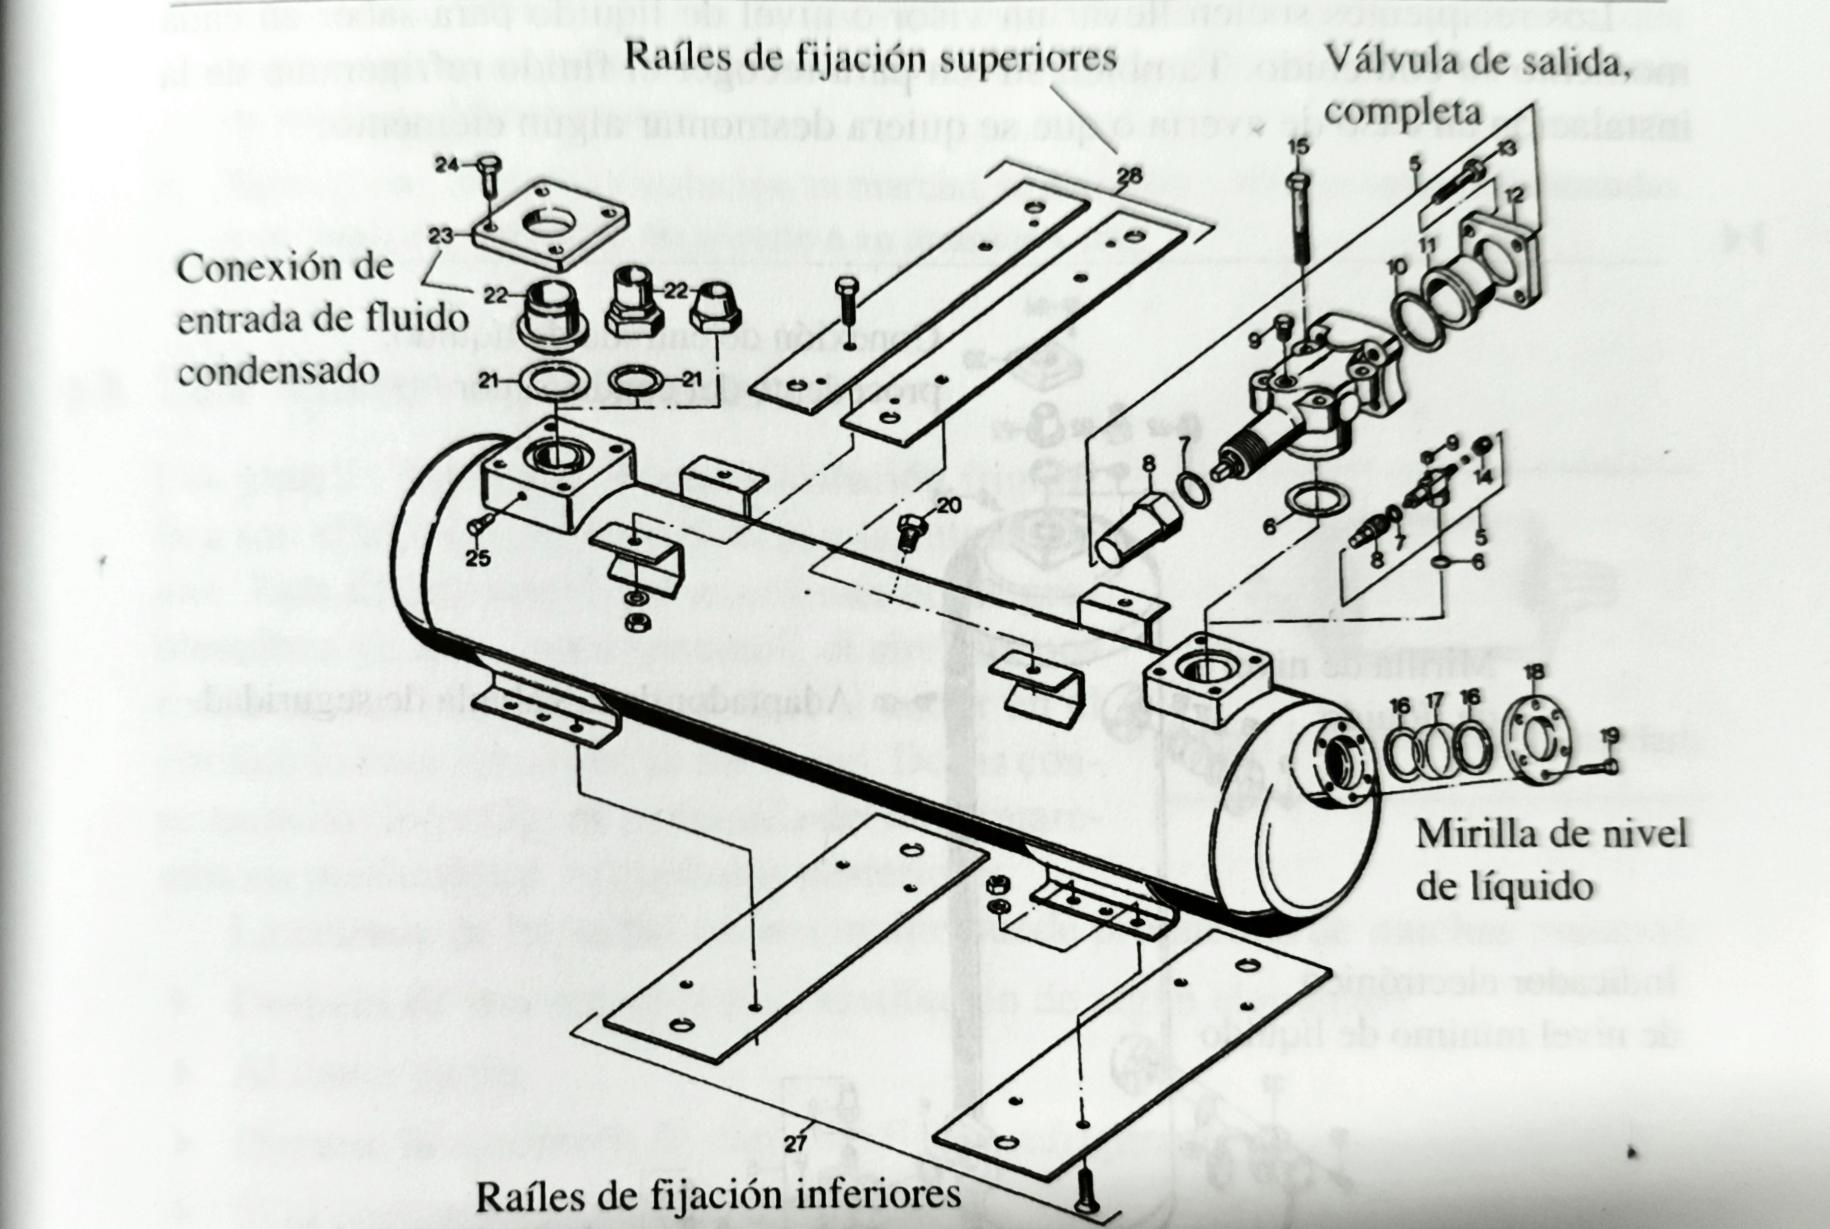
\includegraphics[width=0.7\textwidth]{figuras/recipiente horizontal.jpg}
	\caption{Recipiente de líquido horizontal}
	\label{fig:Recipiente de líquido horizontal}
\end{figure}

Al ser un recipiente de alta presión, debe llevar sus dispositivos de seguridad para evitar que se almacenen presiones peligrosas. También suelen llevar un visor o nivel de líquido para saber en cada momento su contenido.

\subsubsection{Filtros de humedad}

Los grandes enemigos de una instalación frigorífica son el temido golpe de líquido y la entrada de aire. Esta última implica a su vez la doble problemática, como sabemos, el aire que nos rodea es aire húmedo, con lo cual al entrar en el circuito lo hace junto con su humedad.

La entrada de humedad en un circuito puede producirse de muchas maneras:

\begin{itemize}
	\item Después de una reparación (o sustitución de un elemento)
	\item Al meter aceiteDurante la operación de carga de un fluido refrigerante
	\item Si el compresor aspira del aire ambiente
\end{itemize}

La humedad puede ocasionar serios problemas tales como bloquear los dispositivos de expansión (congelación de esas gotas del aire húmedo) o bien producir problemas en los compresores herméticos o semiherméticos, oxidaciones, etc. Para evitar la humedad en los circuitos se instalan unos filtros de humedad también llamados deshidratadores. Contienen un agente desecante que puede ser:

\begin{itemize}
	\item Silicagel
	\item Tamices moleculares
	\item Alúmina activada 
	\item Óxido de aluminio, muy empleado con los nuevos fluidos refrigerantes
\end{itemize}

También existen los denominados núcleo sólido, que son una mezcla de silicagel, tamices moleculares y óxido de aluminio.

Los filtros de humedad además de su función deshidratadora, retienen impurezas (partículas sólidas). 

A la hora de instalarse se deben seguir las intrucciones y el sentido de instalación indicado por el fabricante, si este sentido además es vertical desendente se aumentara el rendimiento del dispositivo.

\textit{La eficacia del agente desecante aumenta cuanto menor sea la temperatura del líquido a la entrada del filtro.} Supongamos, por ejemplo, una instalación con condensador por aire. En verano, al aumentar la temperatura ambiente, también aumenta la temperatura de condensación y por lo tanto la del líquido, lo que influye en la eficacia del agente deshidratador y puede provocar congelación en las válvulas de expansión. Por ello si se debiera instalar un intercambiador de calor, el filtro se montaría después.

\subsubsection{Visor}

De manera práctica diremos que es una ``ventana'' que tenemos en el circuito. A través de él deberíamos ver el fluido en estado líquido 100\% (saturado). Si, por ejemplo vemos burbujas, podría indicarnos que hace falta fluido refrigerante (poca carga, bien sea porque de origen no tiene la adecuada o por fugar posteriores) o bien, si hay burbujar y está frío, puede ser porque un estrangulamiento origina un expansión antes de llegar al visor. También nos indica si hay humedad en el circuit, ya que contiene una sal química higroscópica que reacciona con la humedad y cambia de color (no todos lo tienen).

\subsubsection{Acumulador de aspiración}

Es un elemento que se instala en el lado de baja presión, antes del compresor. Su función consiste en evitar que llegue el fluido en estado líquido al compresor. Es un recipiente metálico, que por lo general suele llevar un tubo de entrada y otro de salida. Evidentemente,\textit{el tubo de entrada se conecta a la tubería que viene del evaporador, y el de salida a la que va al compresor.}

No hay que confundir el acumulador de aspiración con el \textit{separador de líquido}, ya que éste es un elemento de las instaciones de régimen inundado y está perfectamente aislado, pues contiene el fluido expansionado a baja presión y temperatura.

\subsubsection{Intercambiador de calor}

Algunas instalaciones llevan intercambiadores de calor a contracorriente líquido-vapor de aspiración. Es decir, se produce intercambio de calor entre el líquido refrigerante procedente del recipiente y el vapor de salida del evaporador.

\begin{figure}[H]
	\centering
	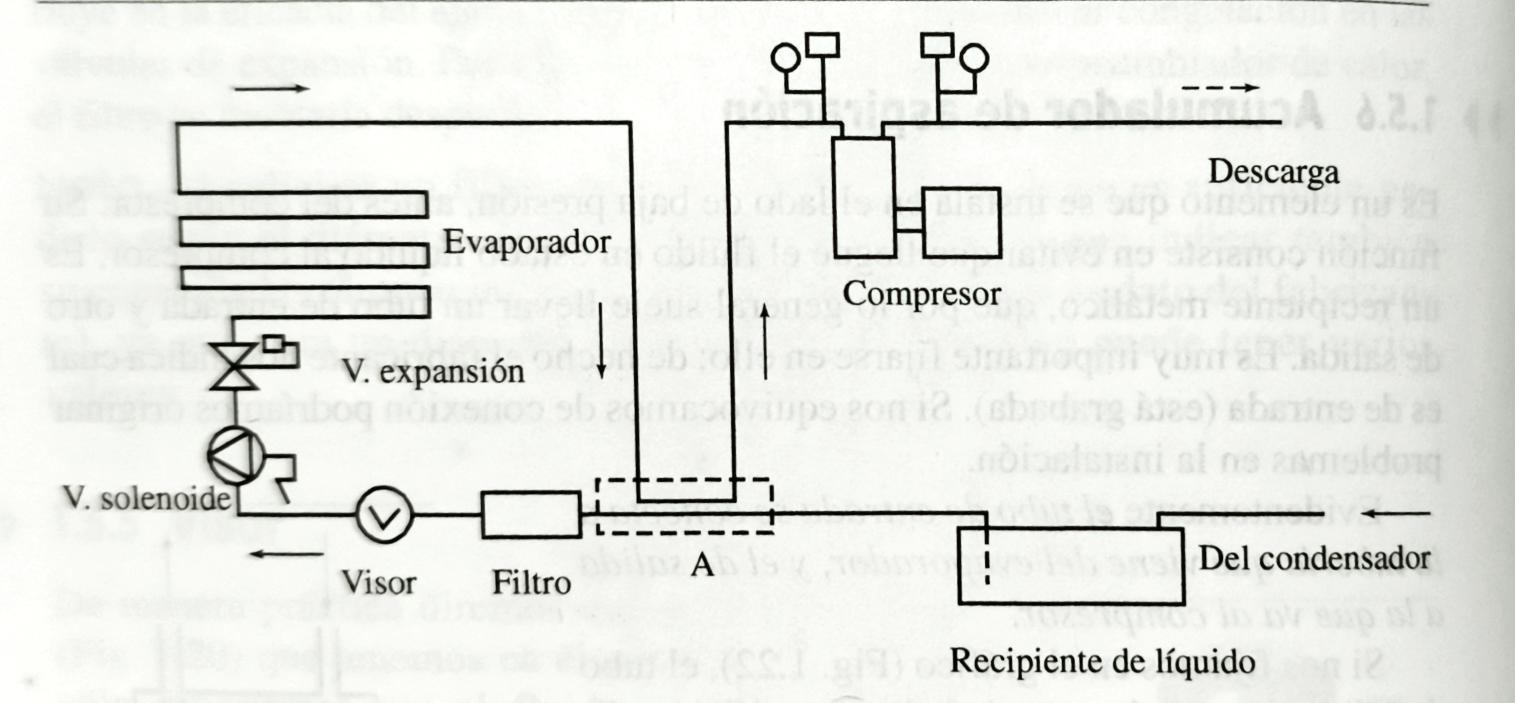
\includegraphics[width=\textwidth]{figuras/instalación con intercambiador.jpg}
	\caption{Instalación con intercambiador de calor}
	\label{fig:Instalación con intercambiador de calor}
\end{figure}

Al ser estos elementos intercambiadores de calor, tienen doble lectura:

\begin{enumerate}[a.]
	\item La del vapor frío de la aspiración que subenfría el líquido que va al dispositivo de expansión y aumenta el rendimiento dado que la temperatura con que entra el líquido en dicho dispositivo es menor (válvula de expansión en la \autoref{fig:Instalación con intercambiador de calor}).
	\item La temperatura del líquido que al estar en contacto con la tubería de salida del evaporador, vaporiza las posibles gotas de líquido que vayan al compresor, es decir evita que llegue líquido al compresor.
\end{enumerate}

